%!TEX root = ../ijcai11storage.tex
\newcommand{\aSet}{\mathname{set}}
\newcommand{\aOperate}{\mathname{operate}}
\newcommand{\aEvaluate}{\mathname{evaluate}}

\newcommand{\pSet}{\mathname{Set*}}
\newcommand{\pSetCharge}{\mathname{SetCharge}}
\newcommand{\pSetDischarge}{\mathname{SetDischarge}}
\newcommand{\pSetNotUsed}{\mathname{SetNotUsed}}
\newcommand{\pExecute}{\mathname{Execute}}

\newcommand{\cSatisfies}{\psi}

\begin{figure*}[t]
\begin{center}
\subfigure[Use case scenario for a modular battery system.]{\label{fig:usecase}
%\resizebox{0.9\columnwidth}{!}{
%!TEX root = ./dp7-application.tex
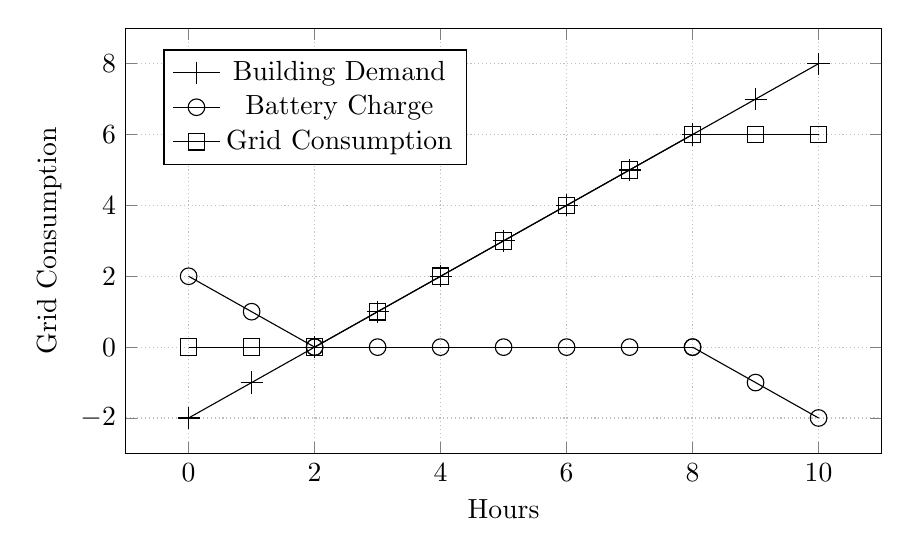
\begin{tikzpicture}

\begin{axis}[
x=0.8cm,y=0.45cm,
xlabel=Hours,
ylabel=Grid Consumption,
grid=both, grid style={style=densely dotted},
legend style={at={(0.05,0.95)},anchor=north west}
] 

% Draw the Demand-Supply curve
\addplot[mark=+,mark size=4] expression[domain=0:10,samples=11] {x-2};
\addlegendentry{Building Demand} 

% Draw the Battery curve
\addplot[mark=o,mark size=3] expression[forget plot,domain=0:2,samples=3] {2-x}; 
\addplot[mark=o,mark size=3] expression[forget plot,domain=2:8,samples=7] {0}; 
\addplot[mark=o,mark size=3] expression[domain=8:10,samples=3] {8-x}; 
\addlegendentry{Battery Charge} 

% Draw the Grid supply curve
\addplot[mark=square,mark size=3] expression[forget plot,domain=0:2,samples=3] {0}; 
\addplot[mark=square,mark size=3] expression[forget plot,domain=2:8,samples=7] {x-2}; 
\addplot[mark=square,mark size=3] expression[domain=8:10,samples=3] {6}; 
\addlegendentry{Grid Consumption} 
\end{axis} 
\end{tikzpicture} 

%}
}
\qquad
\subfigure[Goal-plan hierarchy for a $k$-modules battery system.]{\label{fig:gptree}
%\resizebox{0.9\columnwidth}{!}{
%!TEX root = ../ijcai11storage.tex
\begin{tikzpicture} [level distance=5.5em,child anchor=north]
\tikzstyle{planbox}=[draw,fill=white,text width=5.1em,rectangle split,rectangle split parts=3]
\tikzstyle{goalbox}=[draw,rounded corners=1.25em,minimum height=3em,minimum width=3em]

	
\tikzstyle{level 1}=[sibling distance=6.5em] 
\tikzstyle{level 2}=[level distance=5.5em] 

\node[goalbox,solid] {$G($r,k,s$)$}
	child {node[planbox] {$\pSetCharge$ \\
			\nodepart{second} $k>0$ \\ $\cSatisfies_{ch}(r,k,s)$
			\nodepart{third} $\aSet(k,+c)$
		}
		child {node[goalbox] {$G($r,k-1,s'$)$}}
	}
	child {node[planbox] {$\pSetDischarge$ \\ 
			\nodepart{second} $k>0$ \\ $\cSatisfies_{dc}(r,k,s)$
			\nodepart{third} $\aSet(k,-c)$
		}
		child {node[goalbox] {$G($r,k-1,s'$)$}}
	}
	child {node[planbox] {$\pSetNotUsed$ \\
			\nodepart{second} $k>0$ \\ $\cSatisfies_0(r,k,s)$
			\nodepart{third} $\aSet(k,0)$
		}
		child {node[goalbox] {$G($r,k-1,s'$)$}}
	}
	child {node[planbox] {$\pExecute$ 
			\nodepart{second} $k=0$
			\nodepart{third} $\aOperate()$ \\$\aEvaluate()$
		}
	}
;

\end{tikzpicture}



%}
}
\caption{An energy storage application.}
\end{center}
\label{fig:energystorage}
\end{figure*}
